\section{Challenge Overview}
\label{sec:summary_of_the_crag_challenge}

\subsection{Challenge Tasks}
\begin{figure}[t]
  \centering
  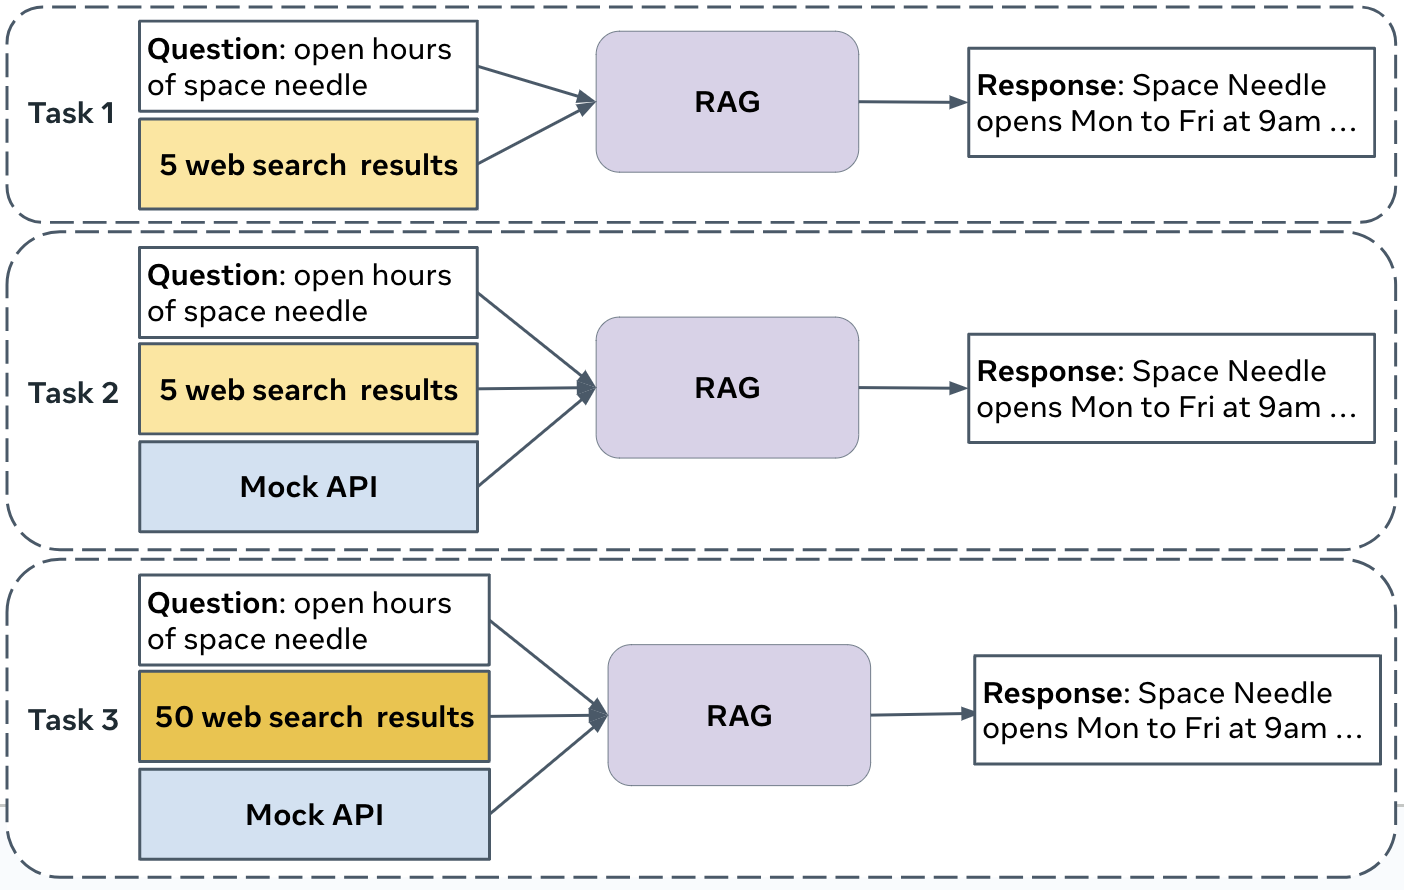
\includegraphics[width=12cm]{submissions/Xiao2024/figs/tasks.png}
  \caption{KDD Cup 2024 Meta CRAG challenge tasks.}
  \label{fig:competition_task}
\end{figure}

A RAG QA system takes a question $Q$ as input and outputs an answer $A$; the answer is generated by LLMs according to information retrieved from external sources or directly from the knowledge internalized in the model. The answer should accurately address the question while avoiding any hallucinations.  


We designed three tasks, which share the same set of (question, answer) pairs but differ in the external data accessible for retrieval to augment QA, as shown in Figure \ref{fig:competition_task}. Here, we provide the content that can be leveraged in QA to ensure fair comparisons.

\noindent
\textbf{Task 1: Retrieval Summarization.} In Task 1, we provide up to five web pages for each question. These web pages are likely, but not guaranteed, to be relevant to the question. This task aims to test the answer generation capability of a RAG system.

\noindent
\textbf{Task 2: KG and Web Retrieval Augmentation.} In Task 2, we in addition provide {\em mock APIs} to access information from underlying {\em mock KGs}. The mock KGs store structured data relevant to the questions; answers to the questions may or may not exist in the mock KGs. The mock APIs take input parameters, oftentimes parsed from the question, and provide structured data from the mocked KGs to support answer generation. This task tests how well a RAG system 1) queries structured data sources and 2) synthesizes information from different sources. 

\noindent
\textbf{Task 3: End-to-end RAG.} Similar to Task 2, Task 3 also provides both web search results and mock APIs as candidates for retrieval but provides $50$ web pages, instead of $5$, as candidates. The larger set of web pages increases the likelihood of providing relevant information to answer the question, but they also tend to contain more noise. As such, Task 3 in addition tests how a RAG system ranks a larger number of retrieval results. 

The three tasks, each adding upon the previous one, allow testing different capabilities of the end-to-end RAG systems. 

\subsection{Data and System Requirement}
The challenge used the CRAG benchmark as described in Section~\ref{sec:intro}. We split the data randomly into {\em validation, public test}, and {\em private test} at 30\%, 30\%, and 40\%, and released the validation and public test sets for the challenge. The final winners were determined by evaluating against the held-out private test set. 

In order to make the systems more comparable and to encourage open source development, we require all submitted systems to be based on Llama 2 \cite{touvron2023llama} or Llama 3~\cite{llama3modelcard} models in this challenge. Participants can also fine-tune their models using publicly available data as long as the data were not generated by proprietary models.

The challenge was hosted on the AICrowd competition platform, and results were posted on a leaderboard. All submissions were run on AWS G4dn.12xlarge instances equipped with 4 NVIDIA T4 GPUs with 16GB GPU memory. Since neither the Llama 2 70B or Llama 3 70B models in full precision can be directly run on these T4 GPUs, participants needed to use quantization or other techniques to make their system runnable on the inference platform. Also, network connection was disabled during the challenge to ensure all participants can access an equal set of retrieved contents, and to prevent leak of the private test set data. Moreover, each example had a time-out limit of 30 seconds and was truncated to 75 BPE tokens~\cite{sennrich-etal-2016-neural} in the auto-evaluation. In human-evaluation, graders examined the first 75 bpe tokens to find valid answers, but reviewed the whole response to judge for hallucination. See section~\ref{sec:evaluation} for more details about the evaluation.


\subsection{Evaluation}
\label{sec:evaluation}

\subsubsection{Metrics}
\label{sec:metrics}
We use a scoring method to assess the performance of RAG systems. For each question in the evaluation set, we first label the answer with \textbf{perfect, acceptable, missing,} or \textbf{hallucination}, according to the following criteria.

\textbf{Perfect.} The response correctly answers the user's question and contains no hallucinated content.

\textbf{Acceptable.} The response provides a useful answer to the user's question but may contain minor errors that do not harm the usefulness of the answer.

\textbf{Missing.} The response is ``I don't know'', ``I'm sorry I can't find ...'', a system error such as an empty response, or a request from the system to clarify the original question.

\textbf{Hallucination.} The response provides wrong or irrelevant information to answer the user's question.
 
We then use a scoring method {\bf Score$_h$} with score $1$, $0.5$, $0$, and $-1$ for each \textit{perfect, acceptable, missing}, and \textit{hallucinated} answer, respectively, where we penalize hallucinated answers because users would prefer the model to admit ``I don't know" than providing an hallucinated answer when it does not know how to answer the question. We then define \textbf{Truthfulness} as the average score from all examples in the evaluation set for a given RAG system. Concretely, 
$$ \text{Truthfulness}_h = \text{Perfect rate} + 0.5 * \text{Acceptable rate} - \text{Hallucination rate}. $$


\subsubsection{Evaluation Method}
\label{sec:evaluation}
We employ a hybrid evaluation system that includes both human evaluation {\bf (human-eval)} and model-based automatic evaluation {\bf (auto-eval)}. In the former, we use manual grading to judge {\em perfect, acceptable, missing}, and {\em hallucinated} for each answer. In the latter, we merge {\em perfect} and {\em acceptable}, call it {\bf accurate}, and use a three-way scoring {\bf Score$_a$} with $1,-1,0$ for {\em accurate}, {\em hallucinated}, and {\em missing} answers. And in this case, 
$$ \text{Truthfulness}_a = \text{Accuracy} - \text{Hallucination rate}. $$

We design a two-step method for automatic evaluation: if the answer matches the ground truth exactly, it is considered {\em accurate}; otherwise, we use LLMs to determine whether the response is {\em accurate, hallucinated}, or {\em missing}. To avoid the {\em self-preference} problem~\cite{panickssery2024llm}, we experimented with two families of LLM evaluators: ChatGPT (\texttt{gpt-3.5-turbo-0125})~\cite{chatgpt2023} and Llama 3 (\texttt{llama-3-70B-instruct})~\cite{llama3modelcard} and reported the average {\em accurate, hallucinated, missing} rates, and scores from the two models for benchmarking the straightforward solutions~\cite{yang2024crag}. This two-step method yields an accuracy of $94.5\%$ for ChatGPT and $99\%$ for Llama 3 compared to human-eval.  We adopted ChatGPT as the auto-evaluator in the challenge due to its low cost.

\subsection{Challenge Schedule and Outcomes}
The challenge was announced on March 15, 2024. Submissions were accepted starting on April 1, 2024, simultaneously with the release of the starter kit. Baseline models were released a week after. The challenge had two phases: in Phase 1, each team can make up to six submissions per week for all three tasks together during a two-month period, and check their results directly on the leaderboard based on auto-eval; in Phase 2, each team can submit up to six times for the three tasks together in total. The submitted solutions in Phase 2 were first evaluated by auto-eval. Then the top-15 teams from each task were sent for human-eval to determine the final winners. Phase 2 ended on June 22, 2024, and the final results were announced on July 28, 2024. 

The challenge awarded the top-3 teams that obtained the highest Truthfulness scores in each task. It also provided seven additional prizes for teams that achieved the highest scores for each of the seven complex question types. In the end, twelve teams won the prizes (See Table~\ref{tab:winning-teams} for the list of the winning teams.), among which six winning teams were invited to present in the KDD 2024 CRAG workshop\footnote{Please see more information about the workshop at: https://kddcup24.github.io/pages/benchmark.html}. All participating teams were encouraged to submit a technical report for their solutions.

The challenge attracted more than 2,500 participants, 384 teams and more than 5,600 submissions. After the challenge was complete, we held a workshop during the ACM KDD 2024 conference. The workshop featured three keynote speeches, six winning-team presentations, and attracted more than 130 onsite audiences. It also published 11 technical reports from the participating teams afterwards.


